\renewcommand{\theequation}{\theenumi}
\begin{enumerate}[label=\thesection.\arabic*.,ref=\thesection.\theenumi]
\numberwithin{equation}{enumi}

\item The trapezium ABCD looks like the Fig. \ref{fig:trapezium_ABCD}.
with $AB \parallel DC$ .AX and BY are perpendiculars to DC drawn from points A and B respectively.


%\renewcommand{\thefigure}{\theenumi.\arabic{figure}}
\begin{figure}[!ht]
\centering
\resizebox{\columnwidth}{!}{%Exercise 8.1 prob 47
\begin{tikzpicture}
[scale=0.5,>=stealth,point/.style={draw,circle,fill = black,inner sep=0.5pt},]
%\tikzset{shift={(-3,0)}}
%Triangle sides
\def\a{4}
\def\c{9}
\def\xA{4}
\def\h{3}
\def\k{1}
%\def\c{7.5}
\def\yE{\h/2}
%Labeling points
\node (D) at (0,0)[point,label=below left:$D$] {};
\node (B) at ({\xA+\a}, \h )[point,label=above right:$B$] {};
\node (C) at (\c, 0)[point,label=below right:$C$] {};
%\node (E) at (2, \yE)
%\node (F) at (8.5, \yE)[point,label=below right:$F$] {};
%\node (M) at (\xA,\yE)[point,label=above right:$M$] {};
%\node (N) at ({\xA+\a}, \yE)[point,label=above left:$N$] {};
%\node (X) at (\xA , 0)[point,label=below left:$X$] {};
%\node (Y) at ({\xA+\a}, 0)[point,label=below right:$Y$] {};
\node (A) at (\xA , \h)[point,label=above left:$A$] {};
\node (E) at ($(D)!0.5!(A)$)[point,label=above left:$E$] {};
\node (F) at ($(B)!0.5!(C)$)[point,label=above right:$F$] {};



%A



%Drawing parallelogram ABCD
\draw (A) -- (B)--(C) --(D)--(A);
%\draw (A) --(X);
\draw (E) --(F);
\draw(A)--node[right]{$\textrm{k}$} (E)--node[right]{$\textrm{1}$} (D);
\draw(B)--node[left]{$\textrm{m}$} (F)--node[left]{$\textrm{1}$} (C);


%\draw (B) --(Y);
%marking right angles
%\tkzMarkRightAngle[fill=green!20,size=.2](D,X,A)
%\tkzMarkRightAngle[fill=green!20,size=.2](C,Y,B)


%
\end{tikzpicture}
}
\caption{Trapezium ABCD by Latex-Tikz}
\label{fig:trapezium_ABCD}	
\end{figure}
%


%
%\renewcommand{\thefigure}{\theenumi}
%
\item List the design parameters for construction
\label{const:table1}
\\
\solution See Table. \ref{table:table1} 
%
\begin{table}[ht!]
\centering
%\begin{tabular}{ |p{3cm}|p{3cm}|  }
%\hline
% \multicolumn{2}{|c|}{Initial Input Values.} \\
%\hline
%\hline
%Length of AB (a) & 4\\
%\hline
%Length of DC (c) & 9\\
%\hline
%Length of AD (d) & 5\\
%\hline
%Height of the trapezium (h) & 3\\
%\hline
%Height at which EF is drawn (k) & 1.5\\
%\hline
%\end{tabular}
%%%%%%%%%%%%%%%%%%%%%%%%%%%%%%%%%%%%%%%%%%%%%%%%%%%%%%%%%%%%%%%%%%%%%%
%%                                                                  %%
%%  This is the header of a LaTeX2e file exported from Gnumeric.    %%
%%                                                                  %%
%%  This file can be compiled as it stands or included in another   %%
%%  LaTeX document. The table is based on the longtable package so  %%
%%  the longtable options (headers, footers...) can be set in the   %%
%%  preamble section below (see PRAMBLE).                           %%
%%                                                                  %%
%%  To include the file in another, the following two lines must be %%
%%  in the including file:                                          %%
%%        \def\inputGnumericTable{}                                 %%
%%  at the beginning of the file and:                               %%
%%        \input{name-of-this-file.tex}                             %%
%%  where the table is to be placed. Note also that the including   %%
%%  file must use the following packages for the table to be        %%
%%  rendered correctly:                                             %%
%%    \usepackage[latin1]{inputenc}                                 %%
%%    \usepackage{color}                                            %%
%%    \usepackage{array}                                            %%
%%    \usepackage{longtable}                                        %%
%%    \usepackage{calc}                                             %%
%%    \usepackage{multirow}                                         %%
%%    \usepackage{hhline}                                           %%
%%    \usepackage{ifthen}                                           %%
%%  optionally (for landscape tables embedded in another document): %%
%%    \usepackage{lscape}                                           %%
%%                                                                  %%
%%%%%%%%%%%%%%%%%%%%%%%%%%%%%%%%%%%%%%%%%%%%%%%%%%%%%%%%%%%%%%%%%%%%%%



%%  This section checks if we are begin input into another file or  %%
%%  the file will be compiled alone. First use a macro taken from   %%
%%  the TeXbook ex 7.7 (suggestion of Han-Wen Nienhuys).            %%
\def\ifundefined#1{\expandafter\ifx\csname#1\endcsname\relax}


%%  Check for the \def token for inputed files. If it is not        %%
%%  defined, the file will be processed as a standalone and the     %%
%%  preamble will be used.                                          %%
\ifundefined{inputGnumericTable}

%%  We must be able to close or not the document at the end.        %%
	\def\gnumericTableEnd{\end{document}}


%%%%%%%%%%%%%%%%%%%%%%%%%%%%%%%%%%%%%%%%%%%%%%%%%%%%%%%%%%%%%%%%%%%%%%
%%                                                                  %%
%%  This is the PREAMBLE. Change these values to get the right      %%
%%  paper size and other niceties.                                  %%
%%                                                                  %%
%%%%%%%%%%%%%%%%%%%%%%%%%%%%%%%%%%%%%%%%%%%%%%%%%%%%%%%%%%%%%%%%%%%%%%

	\documentclass[12pt%
			  %,landscape%
                    ]{report}
       \usepackage[latin1]{inputenc}
       \usepackage{fullpage}
       \usepackage{color}
       \usepackage{array}
       \usepackage{longtable}
       \usepackage{calc}
       \usepackage{multirow}
       \usepackage{hhline}
       \usepackage{ifthen}

	\begin{document}


%%  End of the preamble for the standalone. The next section is for %%
%%  documents which are included into other LaTeX2e files.          %%
\else

%%  We are not a stand alone document. For a regular table, we will %%
%%  have no preamble and only define the closing to mean nothing.   %%
    \def\gnumericTableEnd{}

%%  If we want landscape mode in an embedded document, comment out  %%
%%  the line above and uncomment the two below. The table will      %%
%%  begin on a new page and run in landscape mode.                  %%
%       \def\gnumericTableEnd{\end{landscape}}
%       \begin{landscape}


%%  End of the else clause for this file being \input.              %%
\fi

%%%%%%%%%%%%%%%%%%%%%%%%%%%%%%%%%%%%%%%%%%%%%%%%%%%%%%%%%%%%%%%%%%%%%%
%%                                                                  %%
%%  The rest is the gnumeric table, except for the closing          %%
%%  statement. Changes below will alter the table's appearance.     %%
%%                                                                  %%
%%%%%%%%%%%%%%%%%%%%%%%%%%%%%%%%%%%%%%%%%%%%%%%%%%%%%%%%%%%%%%%%%%%%%%

\providecommand{\gnumericmathit}[1]{#1} 
%%  Uncomment the next line if you would like your numbers to be in %%
%%  italics if they are italizised in the gnumeric table.           %%
%\renewcommand{\gnumericmathit}[1]{\mathit{#1}}
\providecommand{\gnumericPB}[1]%
{\let\gnumericTemp=\\#1\let\\=\gnumericTemp\hspace{0pt}}
 \ifundefined{gnumericTableWidthDefined}
        \newlength{\gnumericTableWidth}
        \newlength{\gnumericTableWidthComplete}
        \newlength{\gnumericMultiRowLength}
        \global\def\gnumericTableWidthDefined{}
 \fi
%% The following setting protects this code from babel shorthands.  %%
 \ifthenelse{\isundefined{\languageshorthands}}{}{\languageshorthands{english}}
%%  The default table format retains the relative column widths of  %%
%%  gnumeric. They can easily be changed to c, r or l. In that case %%
%%  you may want to comment out the next line and uncomment the one %%
%%  thereafter                                                      %%
\providecommand\gnumbox{\makebox[0pt]}
%%\providecommand\gnumbox[1][]{\makebox}

%% to adjust positions in multirow situations                       %%
\setlength{\bigstrutjot}{\jot}
\setlength{\extrarowheight}{\doublerulesep}

%%  The \setlongtables command keeps column widths the same across  %%
%%  pages. Simply comment out next line for varying column widths.  %%
\setlongtables

\setlength\gnumericTableWidth{%
	53pt+%
	53pt+%
0pt}
\def\gumericNumCols{2}
\setlength\gnumericTableWidthComplete{\gnumericTableWidth+%
         \tabcolsep*\gumericNumCols*2+\arrayrulewidth*\gumericNumCols}
\ifthenelse{\lengthtest{\gnumericTableWidthComplete > \linewidth}}%
         {\def\gnumericScale{\ratio{\linewidth-%
                        \tabcolsep*\gumericNumCols*2-%
                        \arrayrulewidth*\gumericNumCols}%
{\gnumericTableWidth}}}%
{\def\gnumericScale{1}}

%%%%%%%%%%%%%%%%%%%%%%%%%%%%%%%%%%%%%%%%%%%%%%%%%%%%%%%%%%%%%%%%%%%%%%
%%                                                                  %%
%% The following are the widths of the various columns. We are      %%
%% defining them here because then they are easier to change.       %%
%% Depending on the cell formats we may use them more than once.    %%
%%                                                                  %%
%%%%%%%%%%%%%%%%%%%%%%%%%%%%%%%%%%%%%%%%%%%%%%%%%%%%%%%%%%%%%%%%%%%%%%

\ifthenelse{\isundefined{\gnumericColA}}{\newlength{\gnumericColA}}{}\settowidth{\gnumericColA}{\begin{tabular}{@{}p{53pt*\gnumericScale}@{}}x\end{tabular}}
\ifthenelse{\isundefined{\gnumericColB}}{\newlength{\gnumericColB}}{}\settowidth{\gnumericColB}{\begin{tabular}{@{}p{53pt*\gnumericScale}@{}}x\end{tabular}}

\begin{tabular}[c]{%
	b{\gnumericColA}%
	b{\gnumericColB}%
	}

%%%%%%%%%%%%%%%%%%%%%%%%%%%%%%%%%%%%%%%%%%%%%%%%%%%%%%%%%%%%%%%%%%%%%%
%%  The longtable options. (Caption, headers... see Goosens, p.124) %%
%	\caption{The Table Caption.}             \\	%
% \hline	% Across the top of the table.
%%  The rest of these options are table rows which are placed on    %%
%%  the first, last or every page. Use \multicolumn if you want.    %%

%%  Header for the first page.                                      %%
%	\multicolumn{2}{c}{The First Header} \\ \hline 
%	\multicolumn{1}{c}{colTag}	%Column 1
%	&\multicolumn{1}{c}{colTag}	\\ \hline %Last column
%	\endfirsthead

%%  The running header definition.                                  %%
%	\hline
%	\multicolumn{2}{l}{\ldots\small\slshape continued} \\ \hline
%	\multicolumn{1}{c}{colTag}	%Column 1
%	&\multicolumn{1}{c}{colTag}	\\ \hline %Last column
%	\endhead

%%  The running footer definition.                                  %%
%	\hline
%	\multicolumn{2}{r}{\small\slshape continued\ldots} \\
%	\endfoot

%%  The ending footer definition.                                   %%
%	\multicolumn{2}{c}{That's all folks} \\ \hline 
%	\endlastfoot
%%%%%%%%%%%%%%%%%%%%%%%%%%%%%%%%%%%%%%%%%%%%%%%%%%%%%%%%%%%%%%%%%%%%%%

\hhline{|-|-}
	 \multicolumn{1}{|p{\gnumericColA}|}%
	{\gnumericPB{\centering}\gnumbox{Parameter}}
	&\multicolumn{1}{p{\gnumericColB}|}%
	{\gnumericPB{\centering}\gnumbox{Value}}
\\
\hhline{|--|}
	 \multicolumn{1}{|p{\gnumericColA}|}%
	{\gnumericPB{\centering}\gnumbox{a}}
	&\multicolumn{1}{p{\gnumericColB}|}%
	{\gnumericPB{\centering}\gnumbox{5}}
\\
\hhline{|--|}
	 \multicolumn{1}{|p{\gnumericColA}|}%
	{\gnumericPB{\centering}\gnumbox{b}}
	&\multicolumn{1}{p{\gnumericColB}|}%
	{\gnumericPB{\centering}\gnumbox{6}}
\\
\hhline{|--|}
	 \multicolumn{1}{|p{\gnumericColA}|}%
	{\gnumericPB{\centering}\gnumbox{c}}
	&\multicolumn{1}{p{\gnumericColB}|}%
	{\gnumericPB{\centering}\gnumbox{4}}
\\
\hhline{|--|}
	 \multicolumn{1}{|p{\gnumericColA}|}%
	{\gnumericPB{\centering}\gnumbox{d}}
	&\multicolumn{1}{p{\gnumericColB}|}%
	{\gnumericPB{\centering}\gnumbox{4}}
\\
\hhline{|-|-|}
\end{tabular}

\ifthenelse{\isundefined{\languageshorthands}}{}{\languageshorthands{\languagename}}
\gnumericTableEnd

\caption{To construct trapezium ABCD}
\label{table:table1}	
\end{table}

%\item

\item Find the coordinates of the various points in Fig. \ref{fig:trapezium_ABCD}
\label{const:trapezium_ABCD}
\\
%
\solution From the given information, 
\begin{align}
\label{eq:constr_d}
\vec{D} &= \myvec{0\\0} 
\\
\vec{C} &= \myvec{0\\c} = \myvec{0\\9} 
\label{eq:constr_c}
\end{align}

$\because \vec{A}$ x coordinate is given , y coordinate is same as the height of the trapezium.  
\begin{align}
\implies \vec{A} &= \myvec{x_a\\h} = \myvec{4\\3}
\label{eq:constr_a}
\end{align}
%
Also, $\vec{B}$ is at a distance a = 4 from $\vec {A}$ and AB is parallel to x axis. 
\begin{align}
\vec{B} &= \myvec{x_b\\h}
\\
AB = \norm{\vec{B}-\vec{A}} = a
\\
\implies a &= \norm{\myvec{x_b\\h} - \myvec{x_a\\h}} 
\\
\implies \norm{\myvec{{x_b - x_a}\\0}} = {x_b - x_a}
\\
%\implies a = x_b - x_a
%\\
\implies x_b = {x_a + a}
\\
\vec{B} &= \myvec{{x_a + a}\\h} = \myvec{8\\3}
\label{eq:constr_b}
\end{align}
%
$\vec{E}$ divides AD in the ratio k: 1. 
\begin{align}
\frac{AD}{ED} = k+1 
\\
\vec{E} &= \frac{{{k\vec{D}} +\vec{A}}}{k+1}
\\
k = 1 \implies \vec{E} & =\myvec{\frac{x_a}{k+1}\\ \frac{h}{k+1}}
\implies \myvec{2\\1.5} 
\label{eq:constr_e}
\end{align}
%
Let $\vec{F}$ divide BC in ratio m:1.
\begin{align}
\vec{F} &= \frac{{{m\vec{C}} +\vec{B}}}{m+1}
\\
\vec{F} &= \myvec{\frac{cm + (x_a + a)}{m+1}\\{\frac{h}{m+1}}}
\label{eq:findm}
\end{align}
EF is parallel to DC and hence the x axis. So we equate y coordinates of E and F to find m.
\\
from \ref{eq:constr_e} and \ref{eq:findm}
\begin{align}
\frac{h}{k+1} = \frac{h}{m+1}
\\
 m = k 
\\
\vec{F} &= \frac{{k\vec{C} +\vec{B}}}{k+1}
\\
\vec{F} &= \myvec{8.5\\3}
\label{eq:constr_f}
\end{align}
%

$\vec{M}$ and $\vec{X}$ have same x coordinate as $\vec{A}$.y coordinate of $\vec{M}$ is same as $\vec{E}$ and y coordinate of $\vec{X}$ is 0
\begin{align}
\vec{M} &= \myvec{x_a\\ \frac{h}{k+1}} = \myvec{4\\1.5}
\label{eq:constr_m}
\end{align}
%
\begin{align}
\vec{X} &= \myvec{x_a\\0} = \myvec{4\\0}
\label{eq:constr_x}
\end{align}
%
$\vec{N}$ and $\vec{Y}$ have same x coordinate as $\vec{B}$.y coordinate of $\vec{N}$ is same as that of $\vec{F}$ and y coordinate of $\vec{Y}$ is 0
\begin{align}
\vec{N} &= \myvec{x_b\\ \frac{h}{k+1}} 
\\
\implies \myvec{{x_a + a}\\ \frac{h}{k+1}} = \myvec{8\\1.5}
\label{eq:constr_n}
\end{align}
%
\begin{align}
\vec{Y} &= \myvec{x_b\\0} =\myvec{x_a + a\\0} =\myvec{8\\0}
\label{eq:constr_y}
\end{align}
The values are listed in \ref{table:table2}. 
%
\begin{table}[ht!]
\centering
\input{./tables/out.tex}
\caption{Derived coordinates trapezium ABCD}
\label{table:table2}	
\end{table}
 
%\item List the  derived values.
%\label{const:table2}
%\\
%\solution See  
%Table. \ref{table:table2} 
%\begin{table}[ht!]
%\centering
%\begin{tabular}{ |p{3cm}|p{3cm}|  }
%\hline
% \multicolumn{2}{|c|}{Derived Values.} \\
%\hline
%$\vec{A}$ & $\begin{pmatrix}4\\3\end{pmatrix}$\\
%\hline
%$\vec{B}$ & $\begin{pmatrix}8\\3\end{pmatrix}$\\
%\hline
%$\vec{E}$ & $\begin{pmatrix}2\\1.5\end{pmatrix}$\\
%\hline
%$\vec{F}$ & $\begin{pmatrix}8.5\\1.5\end{pmatrix}$\\
%\hline
%$\vec{M}$ & $\begin{pmatrix}4\\1.5\end{pmatrix}$\\
%\hline
%$\vec{N}$ & $\begin{pmatrix}8\\1.5\end{pmatrix}$\\
%\hline
%$\vec{X}$ & $\begin{pmatrix}4\\0\end{pmatrix}$\\
%\hline
%$\vec{Y}$ & $\begin{pmatrix}8\\0\end{pmatrix}$\\
%\hline
%\end{tabular}
%\caption{To construct Trapezium ABCD}
%\label{table:table2}
%\end{table}
%
\item Draw Fig. \ref{fig:trapezium_ABCD} using python	
\\
\solution The  following Python code generates Fig. \ref{fig:trapezium_ABCD}
%
\begin{lstlisting}
codes/prob.py
\end{lstlisting}
\begin{figure}[!ht]
\centering
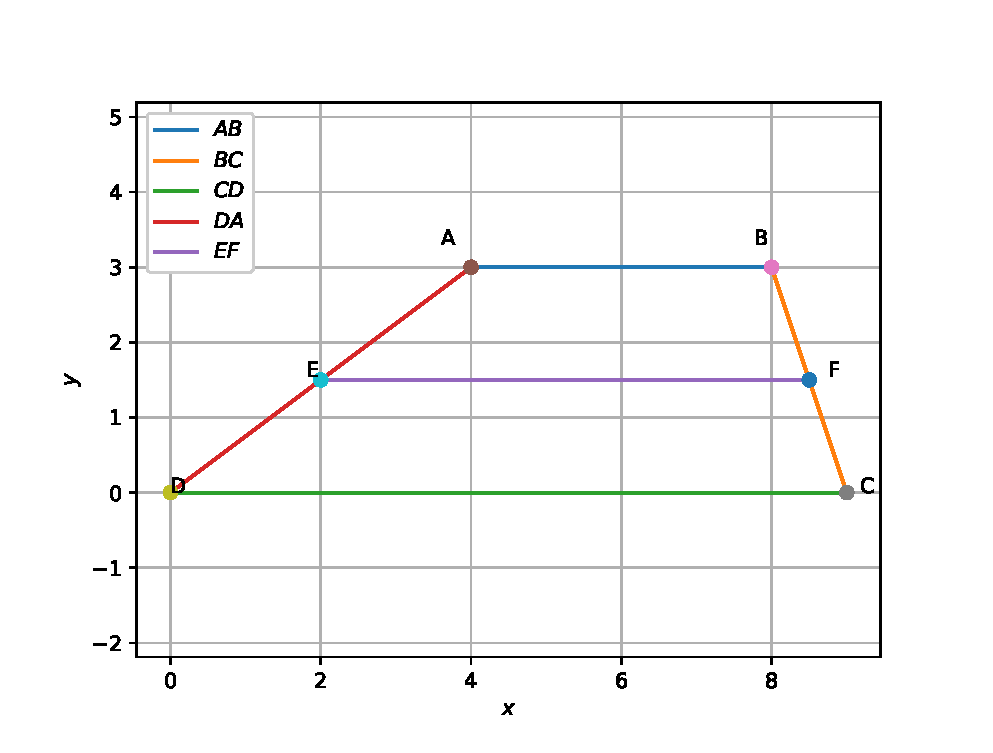
\includegraphics[width=\columnwidth]{./codes/pyfigs/pyfigs.eps}
\caption{Trapezium ABCD generated using python}
\label{fig:trap_py}
\end{figure}

%
and the equivalent latex-tikz code generating Fig. \ref{fig:trapezium_ABCD} is 
\begin{lstlisting}
figs/prob.tex
\end{lstlisting}
%
The above latex code can be compiled as a standalone document as
\begin{lstlisting}
figs/prob_alone.tex
\end{lstlisting}

%

%

%
%

\end{enumerate}
